\documentclass[fontsize=12pt,paper=a4,twoside]{scrartcl}

\usepackage{graphicx}
\usepackage{listings}
\usepackage[ngerman]{babel}

% SWP-Präambel
% C 2003-2017 Sebastian Offermann, Rainer Koschke, Karsten Hölscher
% In Zeilen 40 und 41 sind jeweils die aktuellen Daten einzutragen

\usepackage[utf8]{inputenc}     % Kodierung der Tex-Datei
\usepackage[T1]{fontenc}        % Korrekte Ausgabe von Sonderzeichen (Umlaute)
\usepackage[ngerman]{babel}     % Deutsche Einstellungen [ab \begin{document}]

\usepackage{bibgerm}            % Bibliographie
\usepackage{fancyhdr}           % obere Seitenränder gestalten
\usepackage{float}              % Floats Objekte mit [H] festsetzen
\usepackage{graphicx}           % Graphiken als jpg, png etc. einbinden
\usepackage{moreverb}           % zusätzliche verbatim-Umgebungen
\usepackage{pdflscape}          % PDF-Support für landscape
\usepackage[final]{pdfpages}    % Externe PDFs einbinden
\usepackage{stmaryrd}           % zusätzliche Symbole
\usepackage{supertabular}       % Tabellen über Seitenränder hinaus
\usepackage{tabularx}           % Tabellen mit vorgegebener Breite
\usepackage{url}                % setzt URLs schön mit \url{http://bla.laber.com/~mypage}

%%% Die Reihenfolge der folgenden Pakete muss beibehalten werden:
%%% varioref, hyperref, cleveref, bookmark
% Verweise innerhalb des Dokuments schick mit " ... auf Seite ... "
% automatisch versehen. Dazu \vref{labelname} benutzen
\usepackage[ngerman]{varioref}  % [vor hyperref für korrekte Verweise]
\usepackage[colorlinks=true, pdfstartview=FitV, linkcolor=blue,
            citecolor=blue, urlcolor=blue, hyperfigures=true,
            pdftex=true]{hyperref} % [vor bookmark wegen der Optionen]
\usepackage[ngerman]{cleveref}
\usepackage{bookmark}

\hyphenation{Arbeits-paket}     % Trennungsregeln

%%% Definitionen
\newcommand{\grad}{\ensuremath{^{\circ}} }
\renewcommand{\strut}{\vrule width 0pt height5mm depth2mm}
\newcommand{\gq}[1]{\glqq{}#1\grqq{}}

%%% Semesterkonstanten
\newboolean{langversion} %Deklaration
\setboolean{langversion}{true} %Zuweisung ist 'false' für Blockkurs
\newcommand{\jahr}[1]{2020} %2017/2018

% erstes Argument: SWP-2, zweites SWP-1
\newcommand{\highlight}[1]{\textcolor{blue}{\textbf{#1}}}
\newcommand{\variante}[2]{\ifthenelse{\boolean{langversion}}{#1}{#2}}
\newcommand{\nurlangversion}[0]%
    {\variante{\highlight{}}%Muss in SWP-2 ausgefüllt werden}}%
              {\highlight{Entfällt in SWP-1}}}
\newcommand{\swp}[0]{Software-Projekt \variante{2}{1}}
\newcommand{\semester}[0]{SoSe \jahr}

%%% Formatierungsanpassungen
% Damit Latex nicht zu lange Zeilen produziert:
\sloppy
%Uneinheitlicher unterer Seitenrand:
%\raggedbottom

% Kein Erstzeileneinzug beim Absatzanfang
% Sieht aber nur gut aus, wenn man zwischen Absätzen viel Platz einbaut
\setlength{\parindent}{0ex}

% Abstand zwischen zwei Absätzen
\setlength{\parskip}{1ex}

% Seitenränder für Korrekturen verändern
\addtolength{\evensidemargin}{-1cm}
\addtolength{\oddsidemargin}{1cm}

\bibliographystyle{gerapali}

% 1. Parameter: Euer/Eure TutorIn, z. B. {Kim Harrison}
% 2. Parameter: Abgabedatum, z. B. {05. April 2063}
% 3. Parameter: Versionsnummer, z. B. {1.1}
% 4.-9. Parameter: jeweils Name und (Uni-)Email-Adresse jedes 
%                 Gruppenmitglieds; mit einem & getrennt, z. B.
% {Robin Cowl & roco@tzi.de}
% Besteht die Gruppe aus weniger als 6 Personen, so werden die 
% übrigen Parameter leer gelassen: {}
\newcommand \swpdocument[9] {
% Lustige Header auf den Seiten
  \pagestyle{fancy}
  \setlength{\headheight}{70.55003pt}
  \fancyhead{}
  \fancyhead[LO,RE]{\swp{}\\%
                    \semester{}\\%
                    \documentTitle}
  \fancyhead[LE,RO]{Seite \thepage\\%
                    \slshape \leftmark\\%
                    \slshape \rightmark}

% Lustige Header nur auf dieser Seite (Titelseite)
  \thispagestyle{fancy}
  \fancyhead[LO,RE]{ }
  \fancyhead[LE,RO]{Universität Bremen\\%
                    FB 3 -- Informatik\\%
                    Dr. Karsten Hölscher\\%
                    TutorIn: #1}
  \fancyfoot[C]{}

% Start Titelseite
  \vspace{3cm}
  \begin{minipage}[H]{\textwidth}
    \begin{center}
      \bfseries \Large \swp{} -- \semester{}\\
      \smallskip
      \small VAK 03-BA-901.02\\
      \vspace{3cm}
    \end{center}
  \end{minipage}
  \begin{minipage}[H]{\textwidth}
    \begin{center}
      \vspace{1cm}
      \bfseries \Large \documentTitle\\
      \vfill
    \end{center}
  \end{minipage}
  \vfill
  \begin{minipage}[H]{\textwidth}
    \begin{center}
      \sffamily
      \begin{tabular}{lr}
        #4 \\
        #5 \\
        #6 \\
        #7 \\
        #8 \\
        #9 \\
      \end{tabular}
      \\[22mm]
      \itshape Abgabe: #2 --- Version #3 \\ ~
    \end{center}
  \end{minipage}
% Ende Titelseite

% Start Inhaltsverzeichnis
\newpage
  \thispagestyle{fancy}
  \fancyhead{}
  \fancyhead[LO,RE]{\swp{}\\%
                    \semester{}\\%
                    \documentTitle}
  \fancyhead[LE,RO]{Seite \thepage\\%
                    \slshape \leftmark\\~}
  \fancyfoot{}
  \renewcommand{\headrulewidth}{0.4pt}
  \tableofcontents
% Ende Inhaltsverzeichnis

% Header für alle weiteren Seiten
\newpage
  \fancyhead[LE,RO]{Seite \thepage\\%
                    \slshape \leftmark\\%
                    \slshape \rightmark}

}



\begin{document}

\tableofcontents

\newpage

% ==================== Installation ====================
%\setcounter{chapter}{1}

\section{Installation}

Um das Programm zu installieren, benötigen sie zunächst sowohl eine valide JDK installation, als auch eine Gradle installation. Wenn sie eine der beiden nicht haben, verfolgen sie bitte folgenden zwei Installationsanleitungen. Sollten sie sowohl eine JDK als auch eine Gradle Installation schon haben, so können sie bei Punkt 0.0.3 weiterlesen.

% ==================== JDK INSTALLATION ====================
\subsection{JDK Installation}

Sie benötigen zunächst eine valide JDK Installation. JDK steht für Java Development Kit und wird verwendet um Java Programme zu entwickeln.
Bei unserem Programm können sie eine beliebige JDK mit einer Version von 8+ herunterladen. Wir werden die Vorgehensweise einer Installation von JDK  8 als Beispiel durchführen.

% ==================== WINDOWS ====================
\subsubsection{Windows JDK Installation}

Navigieren sie bitte auf die Webseite https://www.ninite.com . Ninite ist eine Webseite mit welcher man mehrere Programme gleichzeitig automatisiert herunterladen kann. Dort werden sie unter ''Developer Tools'' eine JDK Version mit dem Namen ''JDK (AdoptOpenJDK) x64 8'' sehen. Kreuzen sie die box daneben mit einem Mausclick an. Scrollen sie nun ganz herunter und clicken sie auf den Knopt ''Get Your Ninite''. Führen sie die heruntergeladene Datei aus, welche dann automatisch JDK 8 installieren wird.

\begin{figure}[h!]
\centering
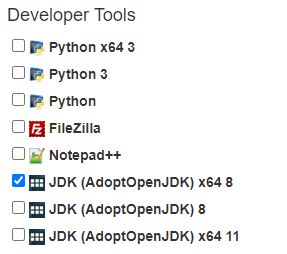
\includegraphics[width=0.5\linewidth]{Windows.JPG}
\end{figure}

Um zu verifizieren das JDK korrekt installiert wurde, öffnen sie ein CMD oder Powershell Fenster, entweder durch ihre Apps oder mit Strg + R, tippen sie dann CMD oder Powershell und drücken sie Enter. Geben sie im geöffneten Fenster das Kommando Javac ein und drücken sie Enter. Sollte nichts passieren, und sie einen Fehler bekommen, so wurde das JDK nicht korrekt installiert und sie müssen das folgende Subkapitel auch noch durchgehen. Wird das Kommando wie im Bild korrekt ausgeführt, so können sie beim Kapitel ''Gradle Installation'' weiterlesen. 

\begin{figure}[h!]
\centering
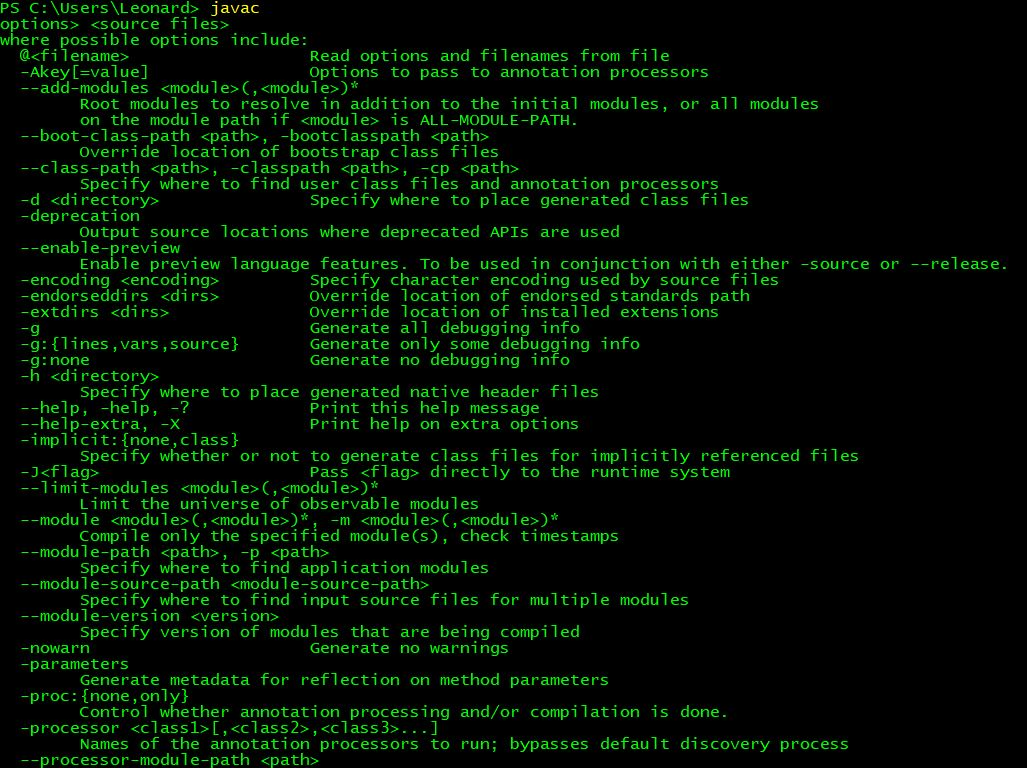
\includegraphics[width=\linewidth]{JavacWindows.JPG}
\end{figure}


\newpage
\paragraph{PATH und JAVA\textunderscore HOME}

Sollte das Kommando im letzten Schritt ein Fehler angezeigt haben, so ist JDK nicht korrekt konfiguriert. Um dieses zu ändern, navigieren sie bitte zu dem Installationspfad ihrer Jdk, welcher einen Namen wie ''C:/Program Files/Java/jdk-version haben wird''. In diesem Ordner werden sie einen weiteren Ordner ''bin'' finden und erst einmal öffnen. Kopieren sie nun den Pfad dieses Ordners (z.B. ''C:/Program Files/Java/jdk-12.0.2/bin'' für JDK 12.0.2) und öffnen sie unter Windows XP/7 My PC, oder unter Windows 8+/10 This PC. Clicken sie die rechte Maustaste und wählen sie ''Properties'' aus.
\begin{figure}[h!]
\centering
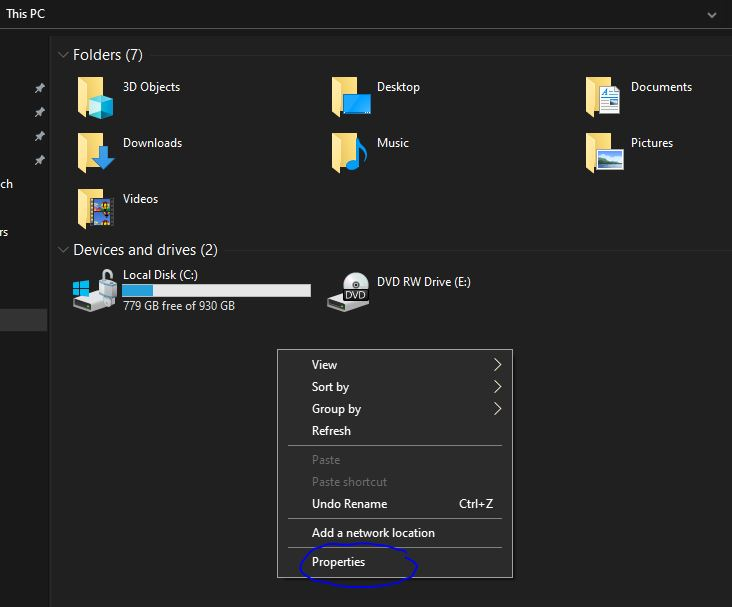
\includegraphics[width=0.7\linewidth]{Properties.JPG}
\end{figure}

In dem geöffneten Fenster auf der linken Seite werden sie einen Knopf ''Advanced System Settings'' sehen, welchen sie nun anclicken.
\begin{figure}[h!]
\centering
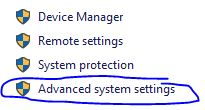
\includegraphics[width=0.5\linewidth]{AdvancedSystemSettings.JPG}
\end{figure}

\newpage
In dem nun geöffneten Fenster, ganz unten Rechts, clicken sie auf den Knopf ''Environment Variables''.
\begin{figure}[H]
\centering
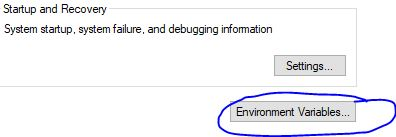
\includegraphics[width=0.5\linewidth]{EnvironmentVariables.JPG}
\end{figure}

Hier sind alle Variablen von Programmen die Windows durch die Konsole erkennt vorhanden. Wr müssen nun unsere JDK Installation dazufügen. Um dieses zu tun, clicken sie bei den ''System Variables'' auf den ''New...'' Knopf und geben der Variable den Namen ''JAVA\textunderscore HOME'', beachten sie das der Name korrekt und groß geschrieben ist, und als Pfad geben sie den kopierten Pfad ohne die ''/bin'' endung an, also z.B. '''C:/Program Files/Java/jdk-12.0.2'' und clicken sie dann auf Ok.
\begin{figure}[H]
\centering
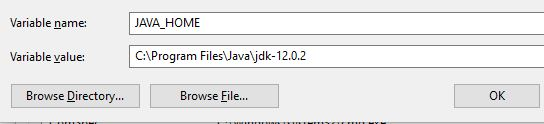
\includegraphics[width=\linewidth]{JAVA_HOME.JPG}
\end{figure} 

\textbf{(*)}
Jetzt müssen sie nur noch ihre System PATH Variable bearbeiten um Java als System Variable einzufügen. Um dieses zu tun, scrollen sie unter ''System Variables'' runter bis sie eine Variable mit dem Namen ''Path'' sehen, und dann diese doppelclicken. In dem jetzt angezeigtem Fenster sind sämtliche Programme die von Windows als System Variablen erkannt werden drin. Clicken sie rechts auf ''New'' und fügen sie den gesamten kopierten Pfad ein und drücken sie Enter. Sie können nun alle Fenster schließen. 
\begin{figure}[H]
\centering
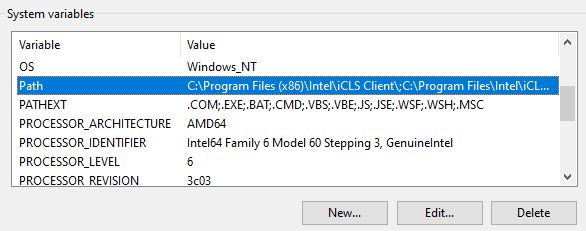
\includegraphics[width=\linewidth]{SystemVariables.JPG}
\end{figure} 

\textbf{(*) Für die Installation auf anderen Betriebssystemen, lesen sie bitte die Dokumentation auf der JDK Oracle Webseite.}

% ==================== LINUX ====================
% TODO ADD LINUX AND MACOS

% ==================== GRADLE INSTALLATION ====================
\subsection{Gradle Installation}

Nun werden wir Gradle installieren. Gradle is ein ein Tool mit welchem man Java Applikationen bauen kann.

% ==================== WINDOWS ======================
\subsubsection{Windows Gradle Installation}

Navigieren sie auf die Webseite https://gradle.org/install/ und scrollen sie runter zu ''Installing manually''. Clicken sie dort auf ''Binary-only'' welches Gradle herunterladen sollte.
\begin{figure}[H]
\centering
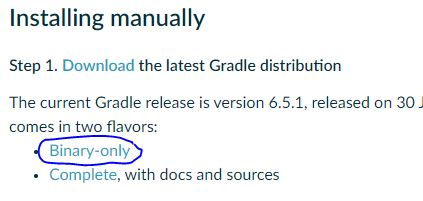
\includegraphics[width=0.5\linewidth]{GradleDownload.JPG}
\end{figure} 

Extrahieren sie die heruntergeladene ZIP datei und kopieren sie den Pfad der bin datei in der Gradle datei, z.B. ''PFAD/gradle-6.4.1/bin'' und erstellen für diesen einen neuen Eintrag in der System Path Variable, siehe (*) bei der JDK Installation. Sie sollten nun die Möglichkeit haben in einem CMD oder Powershell fenster das Kommando ''gradle -version'' ausführen zu können.

\textbf{(*) Für die Installation auf anderen Betriebssystemen, lesen sie bitte die Dokumentation auf der Gradle Webseite.}

% ==================== JRE ====================

\subsection{Java Installation (JRE)}

Um das Programm ausführen zu können, werden sie eine normale Java Installation benötigen. Der Unterschied zwischen der JRE (Java Runtime Environment) und der JDK, ist das die JDK zur Entwicklung von Java Programmen gedacht ist, die JRE aber zur Ausführung dieser Programme benutzt wird. Um die neuste JRE zu installieren, navigieren sie einfach in ihrem Browser auf die Webseite https://www.java.com/download und laden sie sich Java herunter.(Clicken sie einfach immer auf weiter in der Installation)

(*) Wenn sie möchten dass das Programm schneller läuft, so können sie dem mehr Arbeitsspeicher zur Verfügung stellen. Hierbei ist die 32 bit JRE allerdings auf 2GB beschränkt, also könnten sie sich gleich eine 64 bit JRE herunterladen.

% ==================== Application Installation ==================== 

\subsection{Installation der Software}

Nachdem sie nun alle obigen Programme installiert haben, können sie nun endlich die Applikation selbst installieren. Navigieren sie hierzu bitte in den Ordner der Software (galaxytrucker in der Regel), öffnen sie eine Konsole ihrer Wahl und führen sie das Kommando ''gradle clean desktop:dist'' aus. Sollte ihre Gradle Version hiermit Probleme haben, so können sie auch den Projekt begleitendem gradlew File benutzen, indem sie stattdessen das Kommando ''.\textbackslash gradlew clean desktop:dist'' ausführen. (Unter Windows funktioniert letzteres nur in Powershell und nicht in CMD)  
\begin{figure}[h!]
\centering

\includegraphics[width=0.5\linewidth]{command.JPG}
\end{figure} 
\textbf{Der Gradle Build wird zwar viele Warnungen geben, dieses liegt allerdings daran das Gradle nicht versteht wozu die @NonNull tags gedacht sind, also ignorieren sie diese.}

Nachdem sie die Nachricht ''BUILD SUCCESSFUL'' bekommen, können sie die Programmdatei im Unterordner ''desktop$\rightarrow$build$\rightarrow$libs'' finden. Es wird eine Datei vom Format JAR sein und wahrscheinlich den Namen ''desktop-1.0.jar'' haben.

\begin{figure}[h!]
\centering
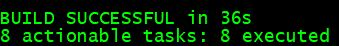
\includegraphics[width=0.5\linewidth]{gradle_build.JPG}
\end{figure} 

\begin{figure}[h!]
\centering
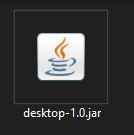
\includegraphics[width=0.5\linewidth]{application.JPG}
\end{figure} 

% ==================== Running Application ==================== 

\subsection{Programmausführung}

Um das Programm nun auszuführen, können sie entweder die JAR durch doppelklick direkt ausführen, oder, wenn sie dem Programm mehr Arbeitsspeicher zur Verfügung stellen wollen (damit es schneller läuft), dieses mit dem Kommando ''java -Xms1G -Xmx4G -jar .\textbackslash desktop-1.0,jar'' starten. Letzteres wird dem Programm mindestens 1 GB Arbeitsspeicher  (Xms steht für Minimum) und bis zu maximal 4 GB Arbeitsspeicher zur Verfügung stellen (Xmx steht für Maximum).

\begin{figure}[h!]
\centering
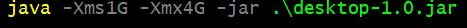
\includegraphics[width=0.8\linewidth]{run_application.JPG}
\end{figure} 

% ==================== The Application ==================== 

\section{Menüs}
Das Menü ist der Ausgangspunkt des Programmes. Hier werden Entscheidungen getroffen die verschiedene Auswirkungen auf die Spielerfahrung haben können.
Das Menü ist in verschiedene Untermenüs aufgeteilt. Durch das Klicken von den entsprechenden Buttons kann man zwischen diesen navigieren.

\subsection{Hauptmenü}
Im Hauptmenü kann man das Spiel starten oder Einstellungen verändern. Die Singleplayer und Multiplayer Buttons führen beide zur Spielauswahl
Sollte bereits ein Spiel im Single- bzw. Multiplayermodus gestartet worden sein, können allerdings nur noch Spiele in demselben Modus gestartet werden, bis das Spiel neu gestartet wird.
Mit Optionen wird das Einstellungsmenü geöffnet.
Quit schließt die Anwendung.

\subsubsection{Spielauswahl}
Auf diesem Bildschirm wird entschieden, ob ein neues Spiel angefangen oder eine begonnene Partie weitergeführt werden soll. New Game leitet direkt zur Schwierigkeitsauswahl weiter. Continue führt zum Ladebildschirm für entweder Single- oder Multiplayer, je nach vorheriger Auswahl.
Mit Back kann zurück ins Hauptmenü gelangt werden.

\subsubsection{Schwierigkeitsauswahl}
\begin{itemize}
\item Easy: Die Leichteste Einstellung für Anfänger oder Spielejournalisten. Gegner machen wenig Schaden.
\item Medium: Normale Einstellung. 
\item Hard: Schwierigste Einstellung. Gegner sind signifikant stärker.
\end {itemize}
Nach der Schwierigkeitsauswahl wird die Schiffauswahl aufgerufen.
Mit Back kann zurück in die Spielauswahl gelangt werden. 

\subsubsection{Schiffsausswahl}
Hier wird das Schiff für das nächste Spiel ausgewählt.
Mit den Pfeilen nach rechts und links kann zwischen den Schiffen hin und her gewechselt werden.
In dem Textfeld wird der Username eingegeben. Der Username fungiert auch als Name des Spiels, unter dem der Spielstand gespeichert wird. Um das Spiel später fortzuführen ist empfehlenswert, sich diesen zu merken. Ein einmal verwendeter Name kann nicht erneut als Spielname verwendet werden, selbst wenn dessen Partie bereits beendet wurde. Der einzige weg um einen Namen wieder freizugeben ist manuell die Datenbank zu löschen, sie wird dann beim nächsten Spielstart neu erstellt.

Die Schiffe geordnet von links nach rechts sind wie folgt:
\begin{itemize}
\item Kestrel: Standardschiff. Ausgeglichene Fähigkeiten. Guter Allrounder.
\item Tank: Fokus auf Defensive. Starke Schilde und viel Leben, aber wenig Startkapital und langsame Antriebe.
\item Killer: Fokus auf Sabotage. Langsame Startwaffe die leicht Crew und Systeme ausschaltet. Hat nur ein Crewmitglied, und kein Medbay, also muss das Crewmitglied beschützt werden. Der maximal entwickelte Autopilot erlaubt das Steuern des Schiffes ohne Pilot während dieser anderweitig beschäftigt ist..
\item Barrage: Fokus auf Offensive. Starkes Waffensystem und drei schnelle Waffen erlauben für stetigen aber kräftigen Beschuss. Nachteile sind wenig Leben, schwache Subsysteme und geringes Startkapital.
\item Stealth: Fokus auf Mobilität. Schwache Offensive und überhaupt keine Schilde, aber hohe Ausweichchance dank des sehr starken Antriebs. Dazu kommen starke Subsysteme, viel Energie und ein hohes Startkapital.
\item Boarder: Fokus auf Strategie. Gute Systeme, aber wenig Energie um sie darauf zu verteilen. Die einzigartigen Waffen sind langsam aber stark und können leicht gegnerische Systeme lahmlegen. Große Besatzung und starkes Medbay helfen die Kontrolle über das Schiffinnere zu behalten. Gutes Crew- und Energiemanagement ist vonnöten um das meiste aus den Systemen zu holen und sich den entscheidenden Vorteil zu verschaffen.

\end {itemize}
Mit continue wählt man das derzeitig angezeigte Schiff. Im Singleplayer-modus beginnt hier das Spiel. Im Multiplayermodus kommt man an dieser Stelle zur Spielersuche.

\subsection{Ladebildschirm}
\begin{itemize}
\item (Multiplayer only) Server Address and Port
Im oberen Textfeld wird die gewünschte IP eingegeben, im unteren der gewünschte Port.
\item Username Hier wird der Spielname der gewünschten gespeicherten Sitzung eingegeben. Ein verlorenes Spiel führt zu einem schwarzen Bild und ein siegreiches Spiel führt zum Boss, aber kann nicht weitergeführt werden.
\item continue: Führt die zum Namen passende Partie als weiter.
\item back: führt zurück zur Spielauswahl.
\item join: führt die Partie eines anderen Servers weiter.

\subsection{Optionen}
Von hier kann man auf eine Reihe von Untermenüs zugreifen, in denen das Spielerlebnis angepasst werden kann.
\begin{itemize}
\item Audio: Führt zu den Ton-Einstellungen
\item Credits: Zeigt eine Liste der Leute, die für dieses Projekt Verantwortung übernehmen wollen
\item Control: Führt zu den Steuerungs-Einstellungen (nicht implementiert)
\item General: Führt zu den Bildschirm-Einstellungen (nicht implementiert)
\item Video: Führt zu den Bildschirm-Einstellungen
\item Back: Führt zurück zum vorherigen Bildschirm
\end {itemize}




\subsection{Multiplayer}

Das Spiel verfügt natürlich auch über eine Multiplayer Funktion. Wenn sie gerade vom Singleplayer Modus ins Hauptmenü gegangen sind, dann müssen sie das Spiel leider neustarten, da ihr singleplayer Server erst dann terminiert, wenn das spiel terminiert wird (Um ohne große Zeitverschwendung schnell ein neues singleplayer Spiel starten zu können). Nach dem Neustart können sie, wie im Singleplayer modus auch, erst ihr Schiff auswählen. Sobald sie zum Fenster mit den Server Adressierungsarten kommen, müssen sie je nach dem welche Art von Multiplayer sie wollen, eine der folgenden drei Punkte befolgen.

\subsubsection{Gleicher PC Multiplayer}
Um Multiplayer auf dem gleichen PC zu spielen, benutzen sie als Adresse des Servers eine der folgenden 3 Optionen. Der Port bleibt ihre Entscheidung, allerdings müssen sie beachten das dieser nicht von ihrem Betriebssystem benutzt wird. 
Adressmöglichkeiten:
\begin{itemize}
\item 0.0.0.0
\item 127.0.0.1
\item localhost
\end{itemize}

Die Adressen sind zwar alle (fast-)identisch, sie können sich allerdings beliebig eine davon auswählen.

\subsubsection{LAN Multiplayer}

Beim LAN Multiplayer können sie mit anderen Spielern auf dem gleichen Netzwerk spielen (auch über mehrere Router die mit dem gleichen Anschluss verbunden sind) müssen sie als Adresse des Servers ihre IPv4 Adresse benutzen. Um diese herauszufinden, öffnen sie eine Konsole ihrer Wahl und benutzen sie das passende Kommando zu ihrem Betriebssystem aus den folgenden Optionen:

\begin{itemize}
\item Unter \textbf{Windows}, das Kommando ''ipconfig''
\item Unter \textbf{Linux/MacOS}, das Kommando ''ifconfig''
\end{itemize}

Der Port bleibt auch hier ihre Entscheidung.

\subsubsection{WAN/Online Multiplayer}

Um Online Mulriplayer zu Spielen, müssen sie als Server Adresse ihre Public IP Address benutzen. Um diese herauszufinden ist es am einfachsten wenn sie eine Webseite wie \textbf{https://www.whatsmyip.org} benutzen. Der Port bleibt auch hier ihre Entscheidung.

\subsubsection{Informationen zu LAN/Online Multiplayer}

Um LAN/Online Multiplayer nutzen zu können, müssen sie ein paar Sachen beachten beachten:

\textbf{LAN:} Unter Windows muss ihr Netzwerk in ihren Network Settings als ein \textbf{Privates Netzwerk} konfiguriert sein, damit sich andere auf dem gleichen Netzwerk mit ihnen verbinden können.

\textbf{WAN/Online:} Zusätzlich zu dem was sie bei LAN Multiplayer beachten müssen, müssen sie ihre Firewall so konfigurieren, das andere PCs sich mit ihrem PC verbinden können. Außerdem müssen sie sehr wahrscheinlich in ihrem Router die Port Forwarding option für ihren PC nutzen. Da es hier aber viele verschiedene Konfigurationen gibt (für Firewall und Port Forwarding) bei denen auch andere Sachen wie ihr Antivirus Programm eine Rolle spielen können, werden wir hier nicht mehr Informationen zu dem Thema geben.

\textbf{Um zu testen} ob man ihren Port sehen kann, können sie das mit der Software enthaltene Programm testConnection benutzen (Bitte nur vor dem Spielstart, da sonst der Spielserver herunterfahren wird). Um dieses zu Nutzen brauchen sie eine Python Version von 3.5+ 

%%%%%%%%%%%%%%%%%%%%%%%%%%%%%%%%%%%%

\section{Das Spiel}
Das Spiel beginnt sobald der hier zusehende Bildschirm mit dem vorher ausgewählten Schiff angezeigt wird. 
\begin{figure}[H]
\centering
\includegraphics[width=0.8\linewidth]{DasSpiel/Ui/game.png}
\end{figure} 

Man selbst startet auf der prozentual generierten Karte immer an einem sogenannten Startplaneten, dieser ist leer und nur du, deine Crew und dein Schiff befinden sich dort. Von hier aus kannst du deine Reise durch das Sternensystem beginnen!  
\\
Von hier aus werden nun alle UI-Elemente näher erklärt und deren Zusammenhang beschrieben.

%allgemeine Erklärung was alles ist

\subsection{Schiff Interface}

Das Schiffsinterface ist in viele Unterpunkte aufgeteilt, welche nun in Bezug auf Spielmechaniken und Schiffs-Indikatoren näher erklärt werden.


%nähere Erklärungen zu allen Punkten

\subsubsection{Schiffinformationen}



\subsubsection{Energiemanagement}


\subsubsection{Waffen}


\subsection{Inventar (Ship)}

Das Inventarfenster kann über den Button Ship geöffnet werden. Über den Close Button unten in der Ecke wird es wieder geschlossen. Es kann normal und während des Kampfes, solange der Spieler am Leben ist geöffnet werden. Während der Pause ist dies nicht möglich. 

\begin{figure}[H]
\centering
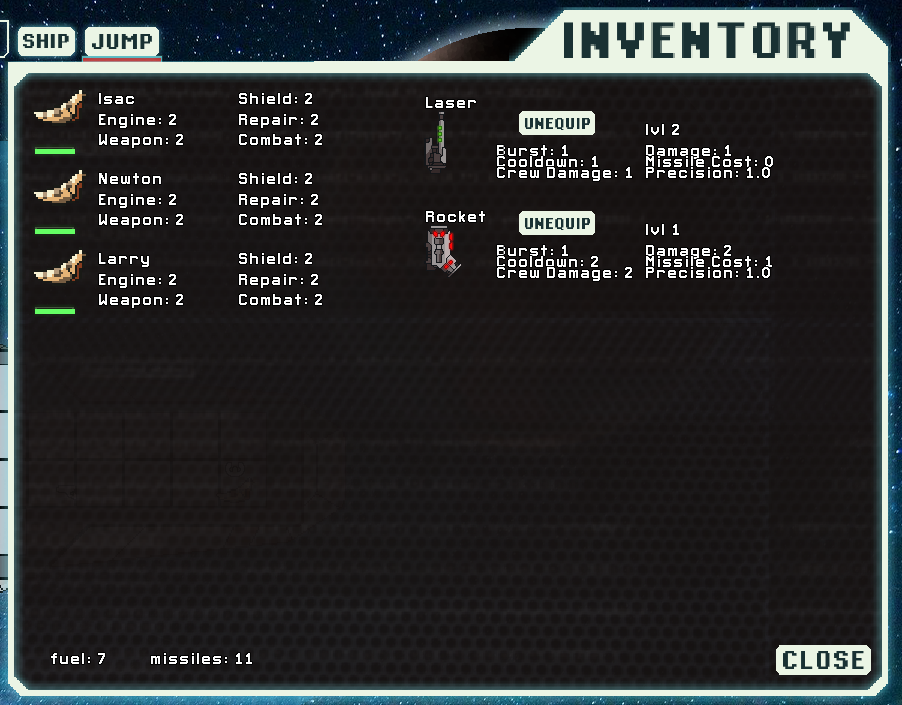
\includegraphics[width=0.8\linewidth]{DasSpiel/Inventar/inventar.png}
\end{figure} 

Auf dem Inventar sieht man unten links (1) die Anzahl an Fuel und die Anzahl der Missiles. Unten Rechts (2) ist der Knopf zum schließen des Fensters. Oben links (3) sieht man seine Crewmitglieder aufgelistet (siehe Crew). Oben rechts sind alle Waffen aufgelistet (siehe Waffen). 

\subsubsection{Crew}

\begin{figure}[H]
\centering
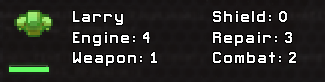
\includegraphics[width=0.8\linewidth]{DasSpiel/Inventar/crew.png}
\end{figure} 

Für jedes Crew Mitglied gibt es ein Anzeigefeld, indem der Name und die Level der Stats des Crewmitglieds angezeigt werden. Von Schiff zu Schiff und wenn man sich im Shop neue Crewmitglieder kauft, haben die unterschiedliche Stats. Man kann Crew nur verlieren, indem sie stirbt. 


\subsubsection{Waffen}

\begin{figure}[H]
\centering
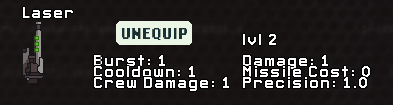
\includegraphics[width=0.8\linewidth]{DasSpiel/Inventar/waffe.png}
\end{figure} 

Für jede Waffe gibt es einen Block, in dem die Informationen der Waffe angezeigt werden. Anhand des Bildes kann man die Klasse der Waffe erkennen. In diesem Beispiel ist das eine Laser Waffe. Außerdem gibt es Raketen, Bomben, Radio und Radiobomben. Jede Waffe hat unterschiedliche Eigenschaften und kann von Lvl 1 bis Lvl 6 gelevelt sein. Über den Equip/Unequip Button kann man die Waffe ausrüsten, oder aus der Ausrüstung herausnehmen. Wenn der Button auf Unequip steht, ist die Waffe ausgerüstet. 



%%%%%%%%%%%%%%%%%%%%%%%%%%%%%%%%%%%%%%%%%%%%%%%%%%%%%%%%%%%%%%%

\subsection{Karte (Jump)}

Das Kartenfenster wird im Spiel mit einem Klick auf den Jump-Button geöffnet. Über den Close Button unten in der Ecke wird es wieder geschlossen. Oben im Fenster sieht man den Map-Schriftzug und die Legende der Symbole.

\begin{figure}[H]
\centering
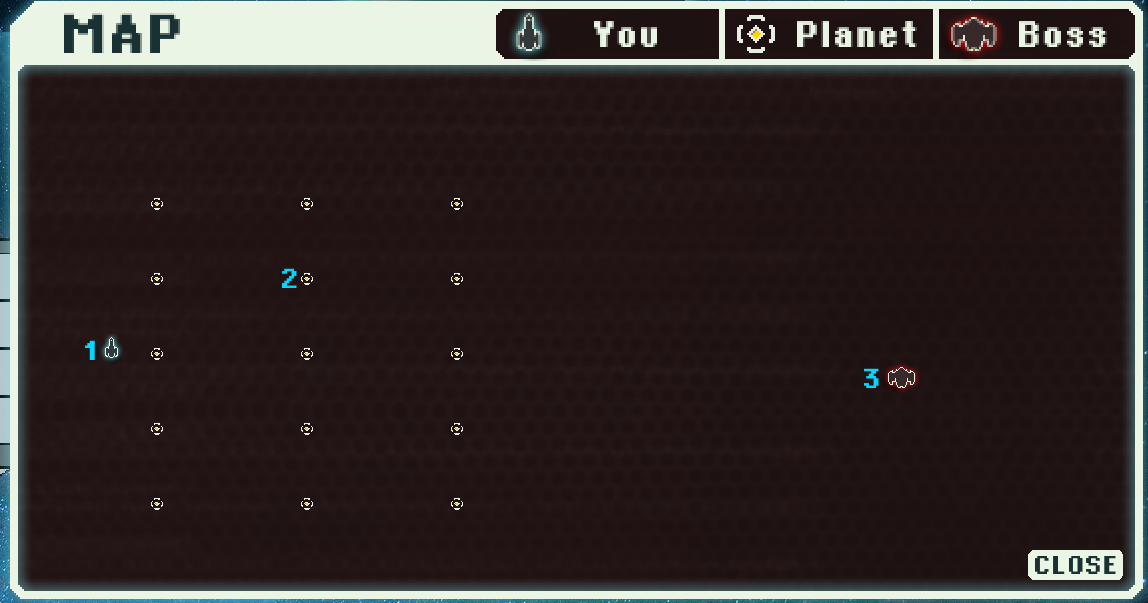
\includegraphics[width=0.8\linewidth]{dasspiel/karte/karteuebersicht.png}
\end{figure} 


Das kleine Schiff (1) Zeigt dem Spieler immer an, auf welchem Planeten er sich gerade Befindet. Hier in dem Beispiel befindet der Spieler sich auf dem Startplaneten. 

Die eingekreisten Punkte (2) sind Planeten, welche das während des Spiels existieren. Bei jedem neu erstellten Spiel wird eine zufällig generierte, einzigartige Karte mit Events auf jedem Planeten erstellt erstellt. 

Das rot hinterlegte Raumschiff (3) ist der Endboss des Spiels. 

\subsubsection{Reisen} 

Das Reisen in diesem Spiel funktioniert nach dem Prinzip, dass ein Planetenwechsel eine Tankeinheit (Fuel) kostet. Grundvorraussetzung ist, dass man ein Crewmitglied im Antrieb und eins im Cockpit hat. Von einem Planeten kann man entweder Vertikal, Horizontal oder Diagonal in alle Richtungen zum nächsten Nachbarplaneten reisen (Siehe Bild unten). Wenn man in der letzten Spalte an Planeten der Map ist, hat man die Möglichkeit, zum Bossplaneten zu reisen.

\begin{figure}[H]
\centering
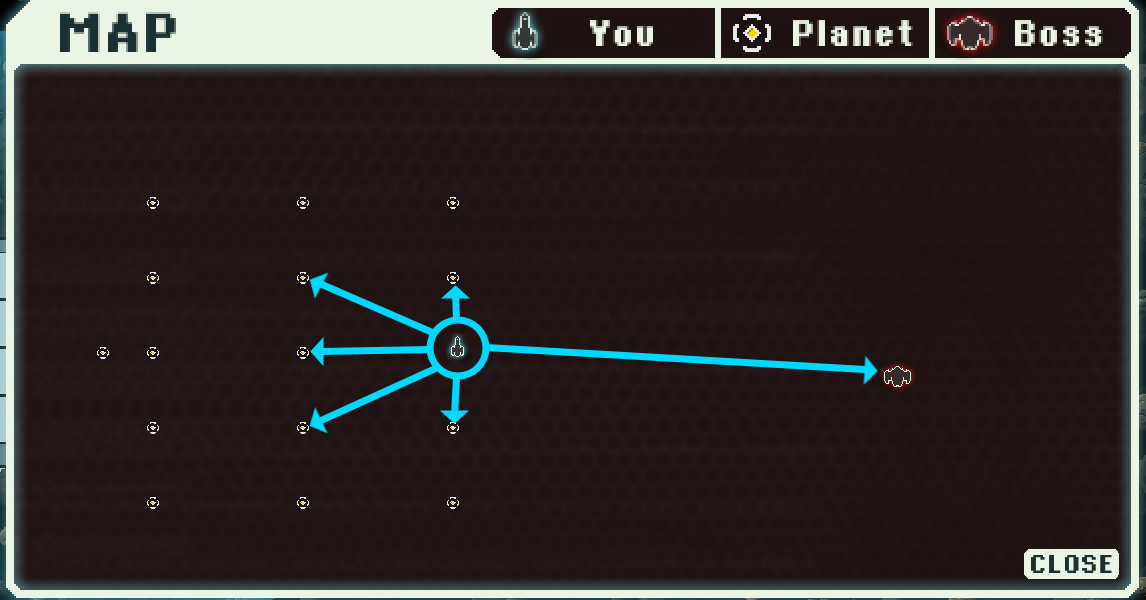
\includegraphics[width=0.8\linewidth]{DasSpiel/Karte/wohinReisen.png}
\caption{Die markierten Stellen können von der aktuellen Position angeflogen werden.}
\end{figure} 




\subsubsection{Planeten}

\paragraph{Startplanet: }
Der Startplanet existiert auf jeder Map nur einmal. Hier gibt es kein Event. Dieser Planet dient dazu, dass man in Ruhe am Anfang des Spiels sich seine Ausrüstung erstmal anschauen kann. 

\paragraph{Normale Planeten: }
Die normalen Planeten sind eine Zufällig generierte Anzahl an Planeten, auf denen Zufällig eins aus 6 Events auftritt (Siehe Events).

\paragraph{Bossplanet: }
Der Bossplanet existiert auf jeder Map nur einmal und ist immer ganz rechts angeordnet. D


\subsubsection{Events}

\subparagraph{Kein Event} Hier Kann es zu einem Zufälligen Geschenk kommen, welches dem Inventar hinzugefügt wird.

\begin{figure}[H]
\centering
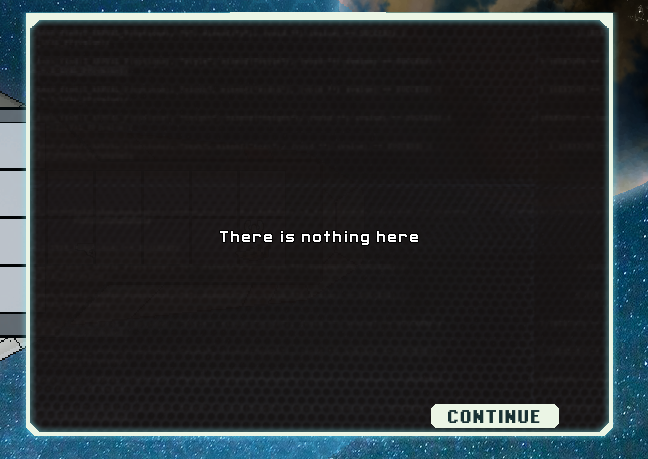
\includegraphics[width=1\linewidth]{DasSpiel/Karte/nothing.png}
\caption{Kein Event Ankunftsmessage}
\end{figure}
 
\subparagraph{Nebel} Hier kann es zufällige Geschenke geben, die dem Spieler zugeschrieben werden.

\begin{figure}[H]
\centering
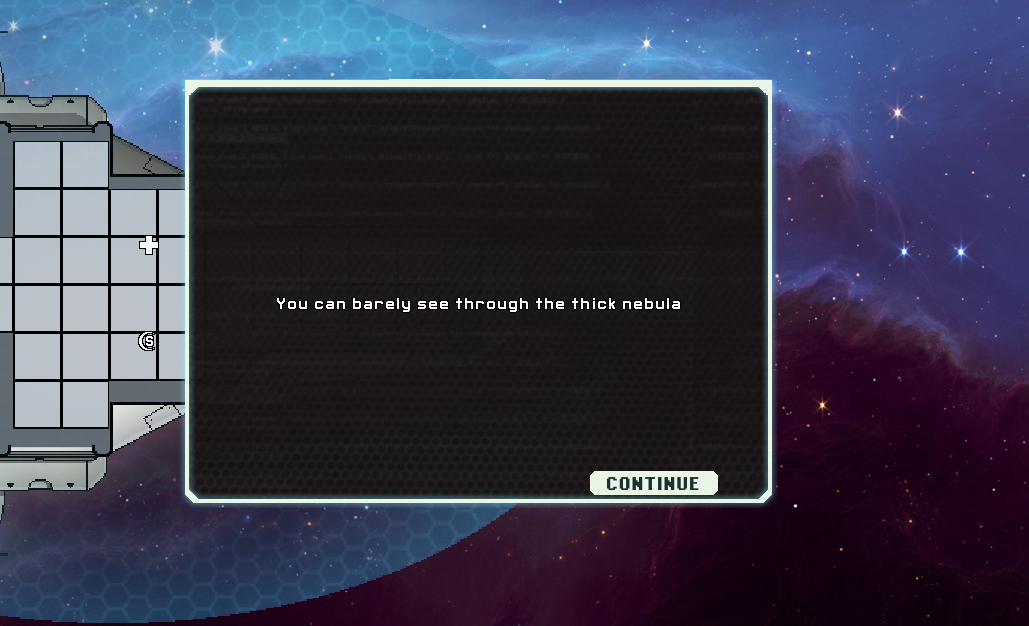
\includegraphics[width=0.8\linewidth]{DasSpiel/Karte/nebular.png}
\caption{Ankunftsnachricht}
\end{figure} 


\begin{figure}[H]
\centering
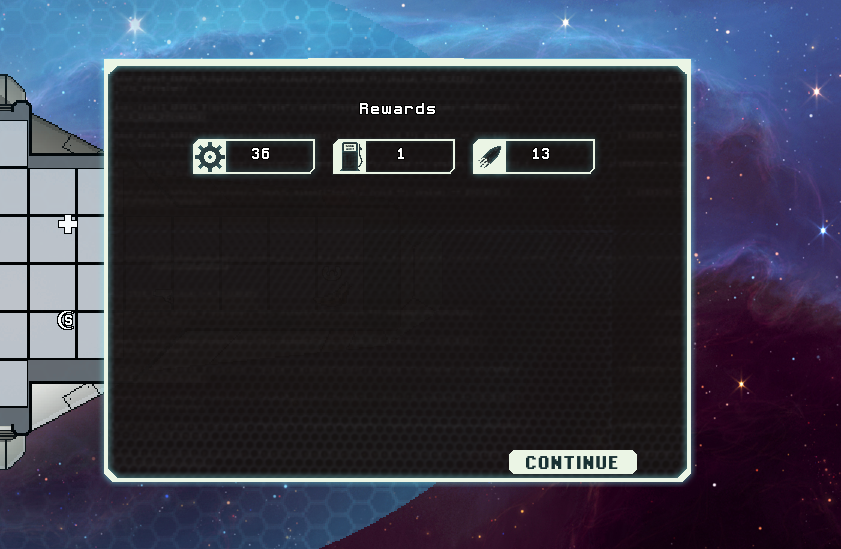
\includegraphics[width=0.8\linewidth]{DasSpiel/Karte/nebularPresent.png}
\caption{Geschenk}
\end{figure} 

\subparagraph{Meteoritenfeld} Hier kann es zu Schäden am Schiff kommen, welche dem Spieler mit Verlust zufälliger Resourcen kenntlich gemacht wird. Es ist außerdem möglich, Zufällige Resourcen zu finden (Geschenk).

\begin{figure}[H]
\centering
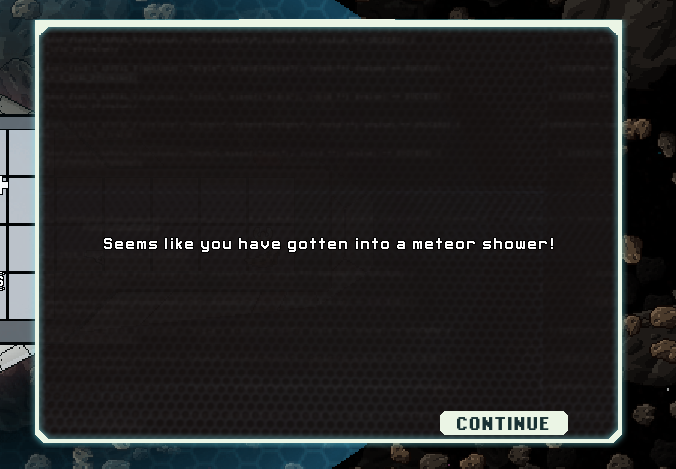
\includegraphics[width=1\linewidth]{DasSpiel/Karte/meteor.png}
\caption{Meteoritenfeld Ankunftsmessage}
\end{figure} 

\begin{figure}[H]
\centering
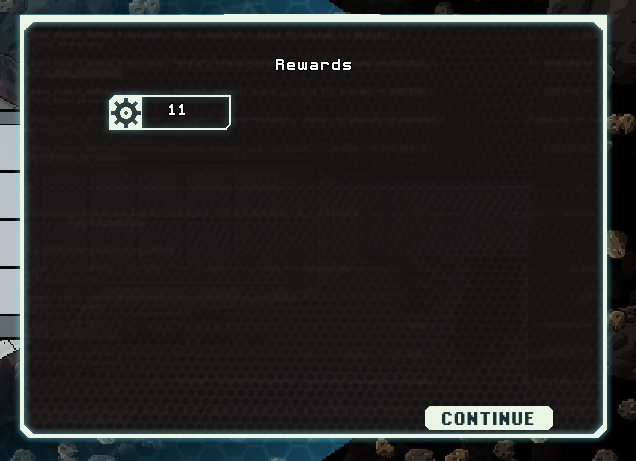
\includegraphics[width=1\linewidth]{DasSpiel/Karte/meteorPresent.png}
\caption{Meteoritenfeld Geschenk}
\end{figure} 



\subparagraph{Gegnerisches Schiff} Hier kann man ein zufälliges Geschenk erhalten. Hier wird ein gegnerisches Schiff angezeigt, welches im folgenden Bekämpft werden muss (Siehe Kampf). Die normalen Gegner haben immer die gleichen Stats und Waffen, welche der Grundausstattung der Schiffe entspricht, aus denen der Spieler auch auswählen kann. Beim Gewinnen bekommt der Spieler eine zufällige Auswahl an Sachen geschenkt. 

\begin{figure}[H]
\centering
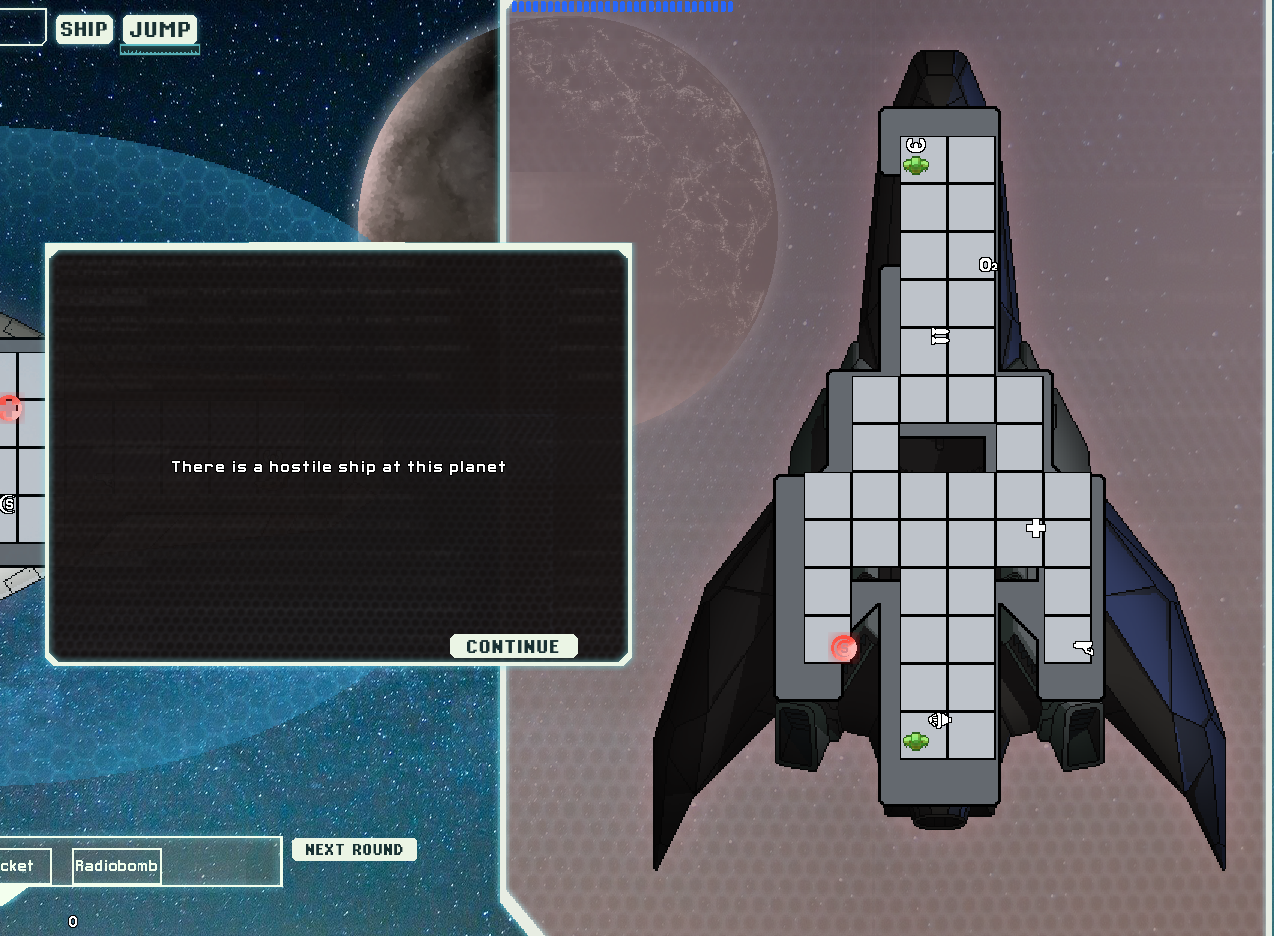
\includegraphics[width=1\linewidth]{DasSpiel/Karte/enemy.png}
\caption{Eins von mehreren gegnerischen Schiffen}
\end{figure} 


\subparagraph{Gegnerisches Schiff (Miniboss)} Das Miniboss Planetevent gleicht dem normalen Gegnerischen Schiff Event, nur dass der Gegner an die Stats des Spielers angepasst wird. Er bekommt ähnlich gute Waffen und ein ähnlich hohes leben, sodass das Besiegen schwerer ist. Beim Gewinnen bekommt der Spieler eine zufällige Auswahl an Sachen geschenkt. 

\begin{figure}[H]
\centering
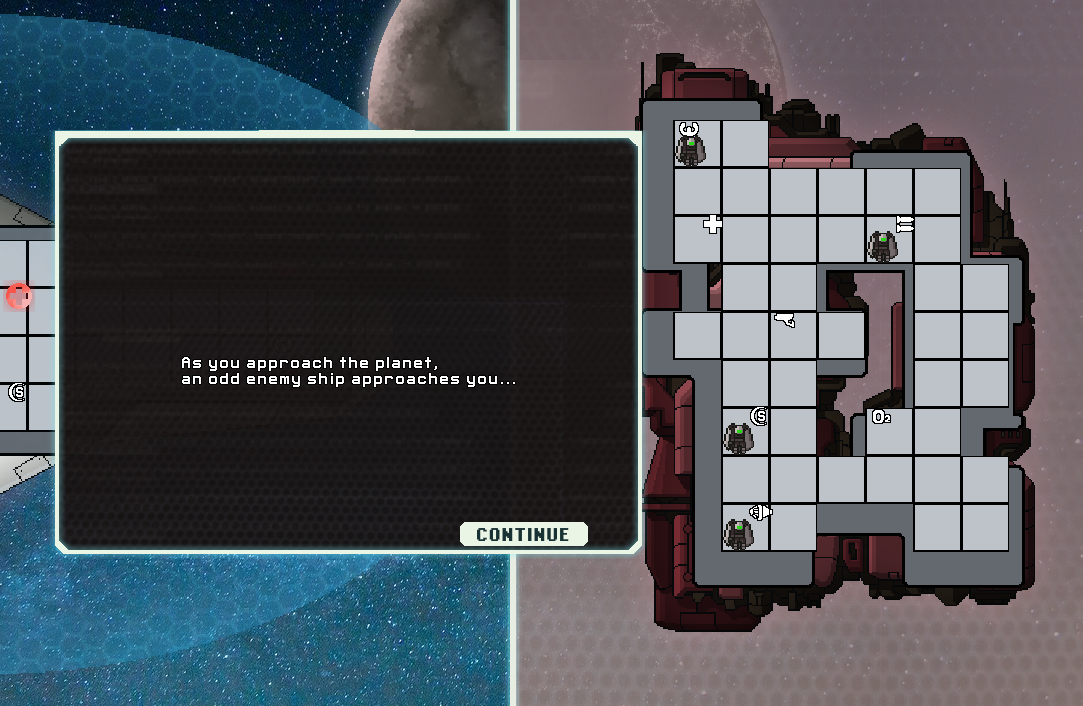
\includegraphics[width=1\linewidth]{DasSpiel/Karte/miniboss.png}
\caption{Der Miniboss hat dieses Schiff mit roter Außenhülle.}
\end{figure} 

\subparagraph{Shop} Beim Shop ist es dem Spieler möglich, Ausrüstung zu kaufen oder zu verkaufen. (Siehe Kapitel Shop)

\begin{figure}[H]
\centering
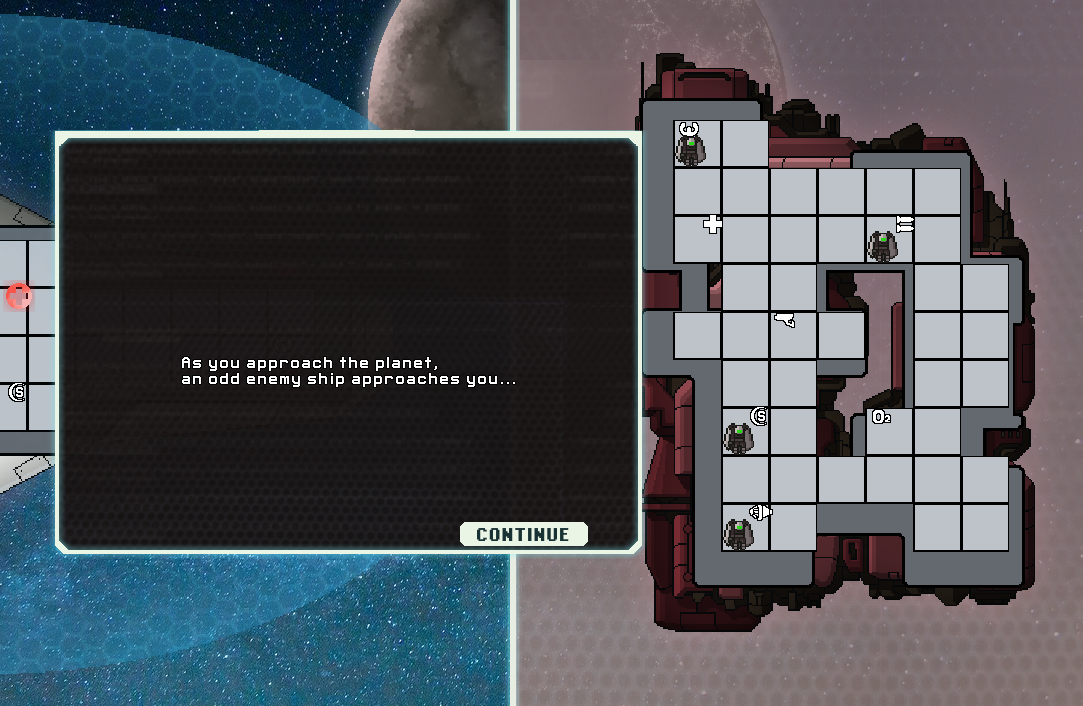
\includegraphics[width=1\linewidth]{DasSpiel/Karte/miniboss.png}
\caption{Shop Ankunftsmessage}
\end{figure}


\subsection{Shop}

Wenn man den Shop öffnet, kommt man auf eine leere Seite. Links sieht man die Tabs Waffen, Resourcen, Crew, Systeme, Upgrades, Verkaufen. Rechts sieht man den Schließen Button. Nun drückt man auf den gewählten Tab und dann öffnet sich der jeweilige Tab. Wenn sich ein leerer Tab öffnet, existiert hier nichts zum Kaufen/Verkaufen. 

\begin{figure}[H]
\centering
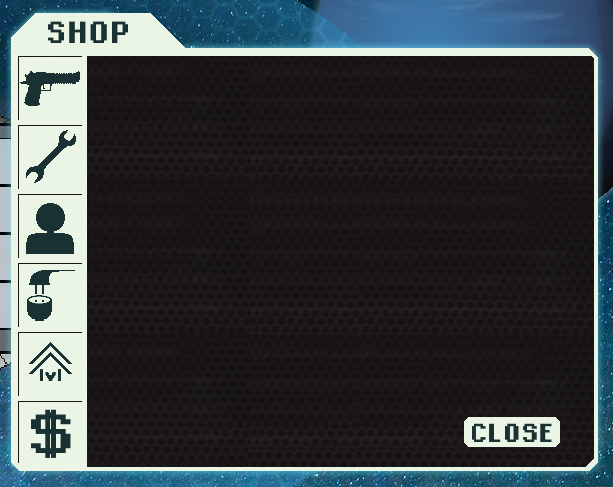
\includegraphics[width=1\linewidth]{DasSpiel/Shop/shop.png}
\caption{Shop Startfenster}
\end{figure}

\subsubsection{Waffen}

Hier sieht man einmal links den Waffentyp anhand des Bildes, In der Mitte steht das jeweilige Waffenlevel und rechts steht der Preis, den der Spieler für die jeweilige Waffe ausgeben muss. Um eine Waffe zu kaufen, drückt man einfach auf das Bild der Waffe. Wenn genug Geld vorhanden ist, verschwindet die Waffe aus dem Shop und ist dann im Inventar. Wenn nicht genügend Geld vorhanden ist, passiert nichts. 

\begin{figure}[H]
\centering
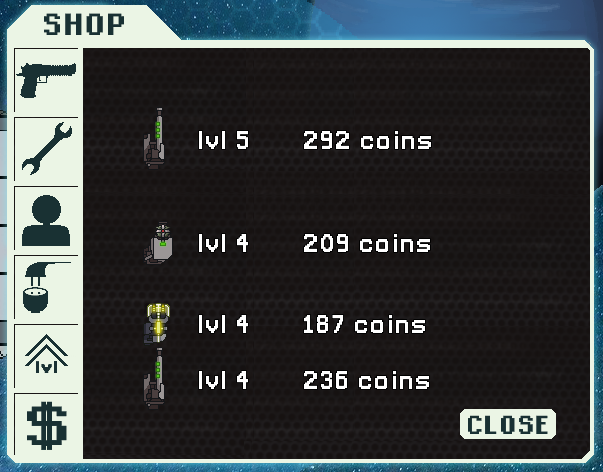
\includegraphics[width=1\linewidth]{DasSpiel/Shop/waffen.png}
\caption{Shop Waffenfenster}
\end{figure}

Sobald man eine Waffe aus dem Shop gekauft hat, wird der Shop nicht mehr restockt. Man kann die selbe Waffe nicht zweimal kaufen. 

\subsubsection{Resourcen}

In Resourcen kann man die drei Hauptresourcen kaufen, Leben (Hull), Raketen (Missiles) und Tank (Fuel). Um eine Resource zu kaufen, muss man auf den grünen Rahmen der Resource klicken. 


\begin{figure}[H]
\centering
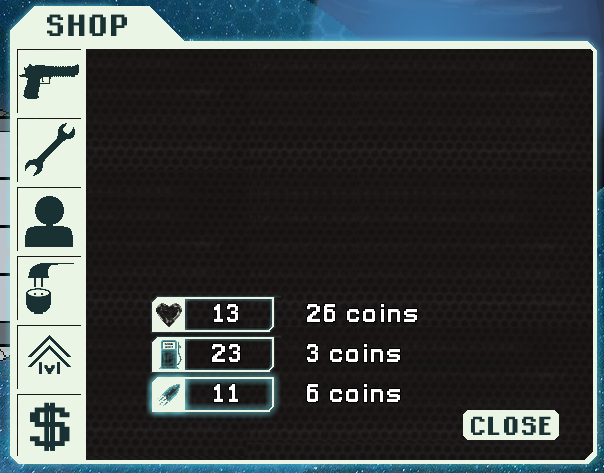
\includegraphics[width=1\linewidth]{DasSpiel/Shop/resourcen.png}
\caption{Shop Resourcenfenster}
\end{figure}

Oben kann man sich Leben (Hull) kaufen. Hier wird eine Anzahl angeboten (In dem Beispiel 13) Und man kann für die 26 Coins direkt alle kaufen. Darunter befindet sich der Tank. In dem Tankschild befindet sich die Anzahl, die der Shop zu verkaufen hat. Für 3 Coins kann man dann eine Tankeinheit kaufen, solange bis die Resource ausverkauft ist. Unten kann man Raketen kaufen. Dies funktioniert analog zu Fuel. 

\subsubsection{Crew}

Im Crewfenster kann man sich neue Crewmitglieder kaufen, welche dann im Schiff auftauchen. 

\begin{figure}[H]
\centering
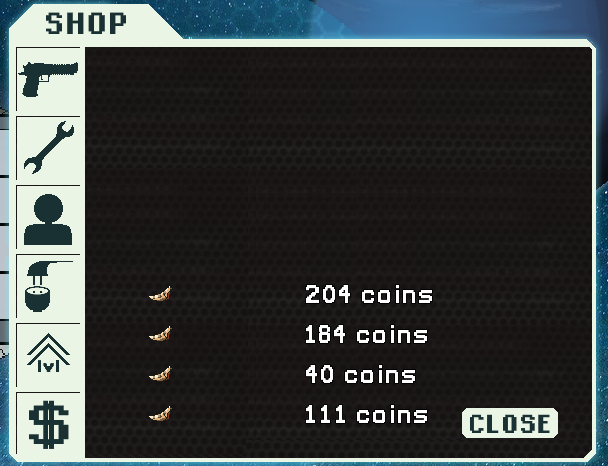
\includegraphics[width=1\linewidth]{DasSpiel/Shop/crew.png}
\caption{Shop Crewfenster}
\end{figure}

Die Crew wird in dem Raumanzug des eigenen Schiffs angezeigt und um diese zu kaufen, muss man auf das Bild klicken. Links neben den Crew Bildern befindet sich jeweils der Preis des Crewmitgliedes. 

\subsubsection{Systeme}

Bei den meisten Schiffen wird hier nichts zu kaufen sein, da die meisten Schiffe schon alle Systeme besitzen. Wenn man ein Schiff mit fehlendem System ausgewählt hat, kann man es hier mit ein wenig Glück nachkaufen. 

\subsubsection{Upgrades}

Hier sieht man die vorhandenen Systeme und kann diese aufrüsten. Das System steht links und rechts steht der Preis. Um es zu kaufen, muss man das Systemlogo anklicken. 

\begin{figure}[H]
\centering
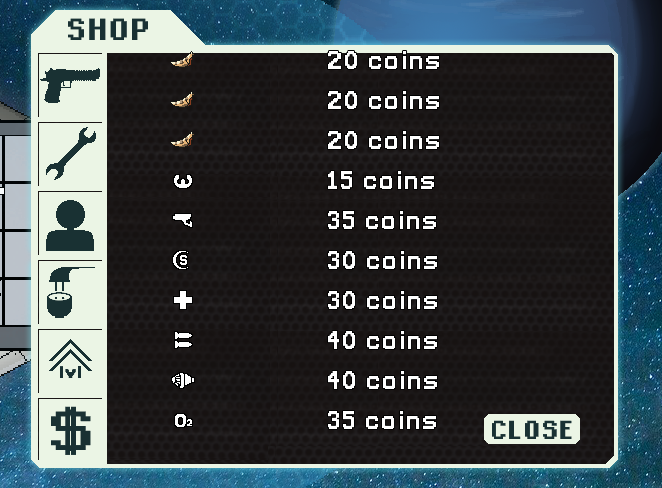
\includegraphics[width=1\linewidth]{DasSpiel/Shop/upgrades.png}
\caption{Shop Upgrades}
\end{figure}

Die Systeme können alle bis zu einem für jedes System festgelegten Wert verbessert werden. 

\subsubsection{Verkaufen}

Das Verkaufen Fenster dient zum Verkaufen der ungenutzten Waffen. Um eine Waffe zu verkaufen, muss man sie im Inventar zunächst unequipen, anschließend taucht die jeweilige Waffe mit ihrem Preis im Verkaufen Fenster auf. Wenn man die Waffe verkaufen will, muss man einfach nur das Bild der jeweiligen Waffe anklicken und erhält das Geld. 

HIER BILD EINFÜGEN AUS NEUEREM BRANCH!!!!!!!!!!

\subsection{Kämpfe}

\subsubsection{Erklärung}

\subsubsection{Mögliche Taktiken}

\subsubsection{Normale Gegner}

\subsubsection{Minibosse}

\subsubsection{Endboss}























\end{document}